\Tsubsection{UI4 Resultados de consulta} 
%------------------------------------Objetivo----------------------------------%
\begin{large}
  \textbf{Objetivo}\\
\end{large}


Permite consultar las noticias clasificadas en la sección previamente elegida. Además brinda una forma de cambiar el periodo de búsqueda y permite entrar al sitio de origen de los artículos mostrados.\\

%------------------------------------Descripción---------------------------------%
\begin{large}
  \textbf{Descripción}\\
\end{large}

La Pantalla \ref{fig:UI4} muestra una sección con las noticias clasificadas, de cada noticia se muestra:

\begin{itemize}

  \item \textbf{Título}
  \item \textbf{URL al artículo}
  \item \textbf{Fecha de publicación}
  \item \textbf{Resumen}

\end{itemize}

En la parte superior de la pantalla se muestra el menú \textbf{Cambio de periodo} el cual permite cambiar le periodo de consulta de las noticias. Cabe señalar que la primera vez que se ingresa a esta pantalla se muestran los artículos con fecha de publicación del día actual.
La Pantalla \ref{fig:UI5} muestra un ejemplo de consulta en una fecha diferente.



%-----------------------------------Salidas------------------------------------%
\begin{large}
  \textbf{Salidas}
\end{large}

\begin{itemize}

  \item \Tref{MSG2}{MSG2 Petición vacía}

\end{itemize}

%------------------------------------Comandos----------------------------------%

\textbf{Comandos}

\begin{enumerate}

  \item \textbf{Hoy}: Realiza la consulta en la fecha actual
  \item \textbf{Ayer}: Realiza la consulta un día antes de la fecha actual
  \item \textbf{Dos días}: Realiza la consulta dos días antes de la fecha actual
  \item \textbf{Tres días}: Realiza la consulta tres días antes de la fecha actual
  \item \textbf{URL}: La url que muestra la noticia direcciona al sitio web de recolección


\end{enumerate}

%------------------------------------Referencia----------------------------------%
\begin{large}
  \textbf{Referenciado por}
\end{large}

\begin{itemize}

  \item \Tref{CU4}{CU4 Mostrar resultados}

\end{itemize}  

%----------------------------------------Pantalla--------------------------------%


%-----------------------------UI1--------------------------%
\begin{figure}[H]\Tlabel{UI4}
  \centering
  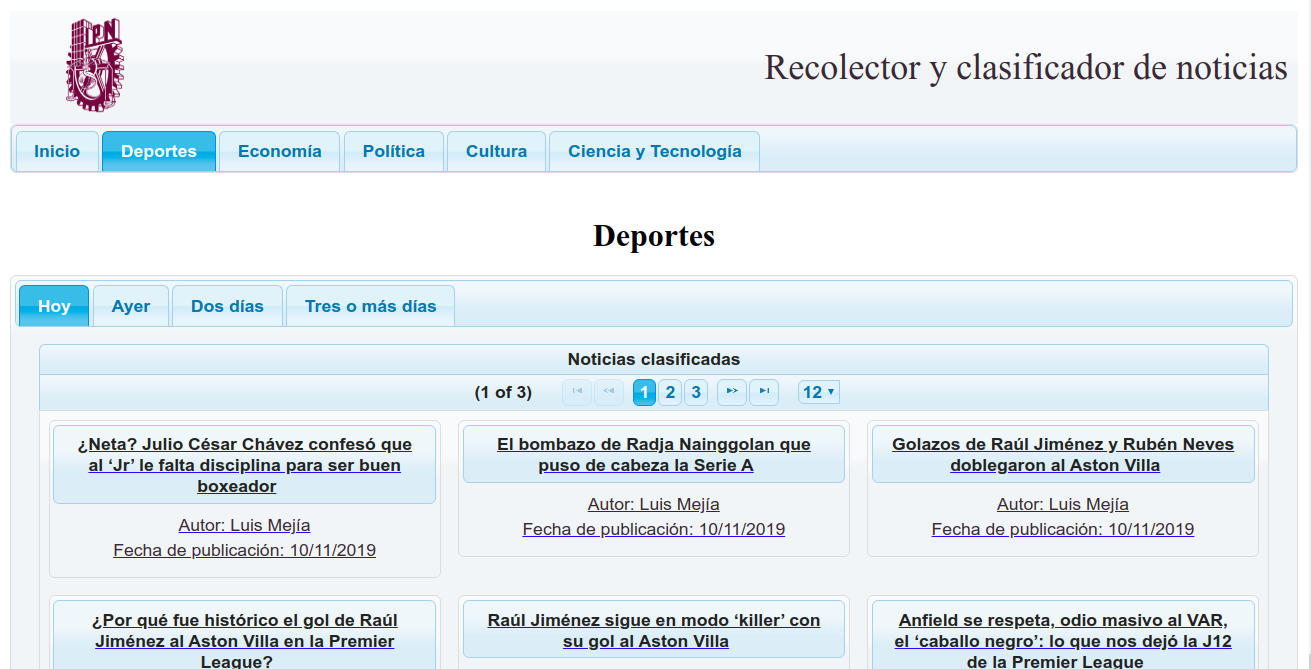
\includegraphics[scale=.4]{imagenes/Pantallas/UI4}
  \caption{Pantalla UI4 Resultados de consulta}
  \label{fig:UI4}
\end{figure}

%-----------------------------UI2--------------------------%
\begin{figure}[H]\Tlabel{UI5}
  \centering
  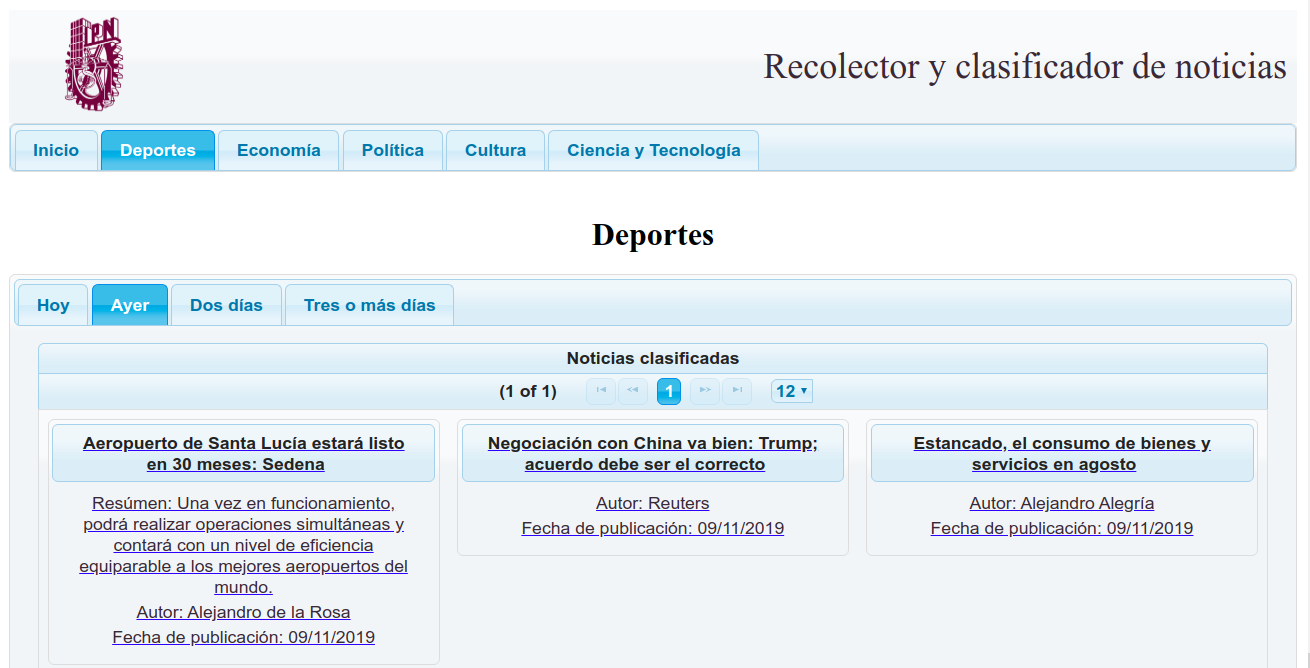
\includegraphics[scale=.4]{imagenes/Pantallas/UI5}
  \caption{Pantalla UI5 Cambio de periodo}
  \label{fig:UI5}
\end{figure}
